\chapter{\IfLanguageName{dutch}{Proof of Concept}{Proof of Concept}}%
\label{ch:PoC}

Dit deel van het onderzoek presenteert een proof of concept gericht op welk framework er gebruik zal worden om machine learning pipelines lokaal uit te voeren, dat gebruikt kan worden in de cursus ``Machine Learning Operations''.
Het doel van deze proof of concept is de efficiëntie en bruikbaarheid van deze frameworks te onderzoeken aan de hand van een lokale opstelling met de gekozen frameworks. Hierbij zal de uitvoering van het framework alsook de resultaten en bevindingen hiervan besproken worden.
Hierna wordt, er aan de hand van de resulaten een conclusie genomen over het gekozen framework.
\section{Vereisten}

% TODO: beschrijf ook de specs van jouw pc, de software-versie, eventuele configuratie en installatie-stappen (of verwijs naar documentatie).

Vooraleer dat er gestart kan worden met het uitwerken van de volgende Proof of Concepts zijn er bepaalde vereisten nodig.
De vereisten zijn als volgt:
\begin{itemize}
    \item Python moet geinstalleerd zijn, Python kan worden geinstalleerd via de documentatie.
    \item De package manager ``pip''
\end{itemize}
Deze vereisten zorgen ervoor dat de volgende hoofdstukken zonder problemen werken.
Als hardwarevereisten is het voldoende voor de minimum vereisten van de opleiding Toegepaste Informatica, als computer.
De Proof of Concept zal ook geen configuratiebestanden veranderen voor de lokale opstelling alles word met de standaard instellingen uitgevoerd.
\section{Ontwikkeling van de Machine Learning pipeline}
% TODO: ik lees vaan "in dit onderdeel", "in dit deel", dat leest moeizaam

In dit onderdeel wordt de opbouw van de Machine Learning pipeline besproken, dit zal er voor zorgen dat het duidelijk is hoe de pipeline in elkaar zit.
De Machine Learning pipeline dat gebruikt gaat worden is die van Labo 3 van de cursus ``Machine Learning Operations''. Deze pipeline is ontworpen om aan de hand van Image Classification het verschil te kunnen herkennen tussen fotos van ``Appelsienen'' en ``Appels'', zoals besproken in de stand van zaken heeft deze pipeline verschillende onderdelen:

\begin{itemize}
    \item Preprocessing: Voor het downloaden en verwerken van de afbeeldingen.
    \item Training: Voor het trainen van het model.
    \item Evaluatie: Voor het evalueren van het moel.
\end{itemize}

De volgende hoofdstukken zullen elk van deze onderdelen toelichten en de werking ervan uitleggen, zoals weergegeven in diagram 1.4.2.
\subsection{Packages}
Dit deel zal alle gebruikte packages kort uitleggen en hoe dat deze geinstelleerd kunnen worden. De packages zijn grotendeels het zelfde voor elke Proof of Concept maar kunnen extra pakcages hebben in verband met het gekozen framework.

De basis packages dat gebruikt zullen worden in de Proof of Concepts zijn:
\begin{itemize}
    \item Tensorflow: Voor het trainen en evalueren van het model, Tensorflow werkt samen met Keras hiervoor.
    \item os: Voor het maken van mappen voor de verschillende datasets die worden gebruikt tijdens de training en de evaluatie van het model.
    \item Requests: Voor het maken van HTTP-verzoeken naar de links van de afbeeldingen om deze dan te kunnen downloaden.
    \item Keras: Voor het maken van het model doormiddel van verschillende lagen.
    \item MLFlow: Voor het bijhouden van alle resultaten van het model, trainingsprocess en de evaluatie.
\end{itemize}

In de bijlage van deze Proof of Concept zal er een bestand zijn genaamd ``requirements\_framework.txt'' worden toegevoegd, waarbij ``framework'' de naam is van het gebruikte framework. Dit bestand kan samen met ``pip'' gebruikt worden om alle packages te installeren met het volgende commando:

\begin{minted}[frame=lines,breaklines,linenos]{bash}
    pip install -r "requirements.txt"
\end{minted}
\section{Virtuele omgeving}

% TODO: Waarom geen virtuele omgeving voor elke tool apart of voor alle tools samen?
% TODO: verplaats het opzetten van de testomgeving naar vooraan dit hoofdstuk, tenzij specifieke vereisten nodig zijn voor de verschillende tools

De volgende hoodstukken zullen gebruik maken van verschillende frameworks, deze frameworks hebben allemaal de mogelijkheid om lokaal een Machine Learning pipeline uit te voeren en deze voldoen ook aan alle nodige criteria van het requirementsanalyse.

Voor elke framework dat gebruikt zal worden word er een virtuele omgeving opgesteld. Dit zorgt ervoor dat er geen conflicten zijn tussen de verschillende versies van de libaries.

\subsection{Preprocessing}
Het Preprocessing gedeelte van de pipeline gaat de data voorbereiden zodat het trainen van het model. Dit omvat het het laden en transformeren van de afbeeldingen, zodat deze afbeeldingen gebruikt kunnen worden als invoer voor het trainen van het model. In dit Proof of Concept wordt er gebruikt gemaakt van Tensorflow's ImageDataGenerator om afbeeldingen in te laden, te normalizeren en te voorzien van labels gebaseerd op de mapstructuur. Na het inladen van de afbeeldingen en deze klaar te maken voor het trainen van het model worden de afbeeldingen gesplits in trainings-, validatie- en testsets. In elke van deze sets worden de juiste labels voorzien. figuur x.x toont aan hoe het er voor deze Proof of Concept eruit zal zien. 
\subsection{Training}
Het Training gedeelte is gaat weldegelijk een Machine Learning-model trainen. Deze Proof of Concept zal gebruik maken van een Convolutional Neural Network (CNN) met behulp van Keras. Dit model bevat verschillende lagen en parameters.
Er word gebruik gemaakt keras sequential model, dit betekend dat alle lagen worden achtereenvolgens worden uitgevoerd. De volgorde en de lagen die gebruikt worden voor dit Proof of Concept zijn als volgend:
\begin{itemize}
    \item Convolutionele laag (Conv2D)
    \item Activatielaag (Activation)
    \item Flatten-laag
    \item Dense-laag
\end{itemize}
\subsection{Evaluatie}
Het evaluatie gedeelte zal het model evalueren dat we hiervoor hebben getraint. Alle resulataten hiervan zullen bijgehouden worden met MLFlow. De resultaten bevatten:
\begin{itemize}
    \item Parameters van het model
    \item systeemeigenschappen en performance
    \item Accuracy van het model en de evaluatie
\end{itemize}

\section{MLflow}
Elk van deze Proof of Concepts bevat MLflow zoals besproken in heeft dit framework heel wat functionaliteiten, voor deze Proof of Concepts gaan we vooral de parameters van het model, de resultaten van de training en de resultaten van de evaluatie bijhouden.
Dit noemt Experiment Tracking, en stelt ons in staat om experimenten bij te houden.

Om van MLflow gebruikt te kunnen maken moeten we het eerst importeren hieronder is een codevoorbeeld hoe dit gebeurd:

Nadata MLflow geimporteerd is, moeten we alle variablen veranderen zodat deze de resulaten naar de juiste server worden gestuurd en de juiste resulaten worden bijgehouden.
De varaiablen die we moeten bijhouden zijn als volgt:
\begin{minted}[frame=lines,breaklines, linenos]{python}
    import mlflow
    import mlflow.keras
\end{minted}

\begin{itemize}
    \item Parameter Logging: Het commando hiervoor is ``mflow().log\_param''. Dit houdts alle parameters bij van het model, zoals het aantal epochs of de batchgrootte.
    \item Metric Logging: Tijdens het trainen van het model zal MLflow belangerijke resulaten bijhouden, zoals de nauwkeurigheid en het verlies van het model. Dit word aan de hand van ``mlflow.log\_metric()'' bijgehouden. Deze metrics worden voor elke epoch van het trainingsproces bijgehouden om het verloop van de training te analyseren.
    \item 
\end{itemize}

\section{Prefect}
Dit deel zal het Proof of Concept uitleggen waarbij Prefect word gebruikt samen met MLFlow voor het lokaal uitvoeren van Machine Learning pipelines, hierbij worden alle aanpassingen uitgelegd in de code van het framework vergeleken met de orignele code van Labo 3 van de cursus ``Machine Learning Operations''
\subsection{Installatie}
De installatie van Prefect gebruikt met de package manager ``pip''. Via de terminal kan je met het volgende commando Prefect installeren, dit zal alle nodige libraries installeren voor deze Proof of Concept.
\begin{minted}[frame=lines,breaklines,linenos]{bash}
    pip install -r "requirements.txt"
\end{minted}

Om enkel Prefect te installeren kan dit met het voglende ``pip'' commando:
\begin{minted}[frame=lines,breaklines,linenos]{bash}
    pip install prefect
\end{minted}

\subsection{Lokale Server}
Prefect heeft de mogelijkheid om Machine Learning pipelines lokaal uit te voeren, dit is aan de hand van een lokale server. 
Deze server kan opgestart worden met het commando: 
\begin{minted}[frame=lines,breaklines,linenos]{bash}
    prefect server start
\end{minted}

% TODO: het resulaat van Figuur~\ref{fig:Prefect_server}
% je moet er dus zelf nog Figuur bij schrijven!

Na het uitvoeren van het start commando zou het resulaat van figuur \ref{fig:Prefect_server} te zien moeten zijn.
\begin{figure}[]
    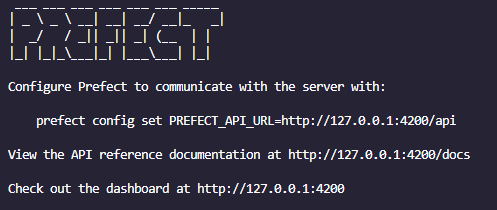
\includegraphics[width=\linewidth]{graphics/Prefect_server.PNG}
    \caption{Prefect Dashboard}
    \label{fig:Prefect_server}
\end{figure}
Nu dat de server is opgestart moet de code nog communiceren met de Prefect web interface. 
Zoals figuut 2 aantoont word dit aan de hand van een commando ingesteld, het maak gebruikt van een lokale API:
\begin{minted}[frame=lines,breaklines,linenos]{bash}
    prefect config set PREFECT_API_URL=http://127.0.0.1:4200/api
\end{minted}
Nu dat de server is opgestart en verbonden in met de lokale omgeving, kan via de link die eerder werd ingesteld het Prefect dashboard bezocht worden.
\subsection{Dashboard}
Het dashboard van Prefect is een omgeving waar alle pipeline flows beheerd worden. Figuur \ref{fig:Prefect_Dashboard} toont aan hoe dat het Prefect dashboard eruit ziet.
\begin{figure}[h]
    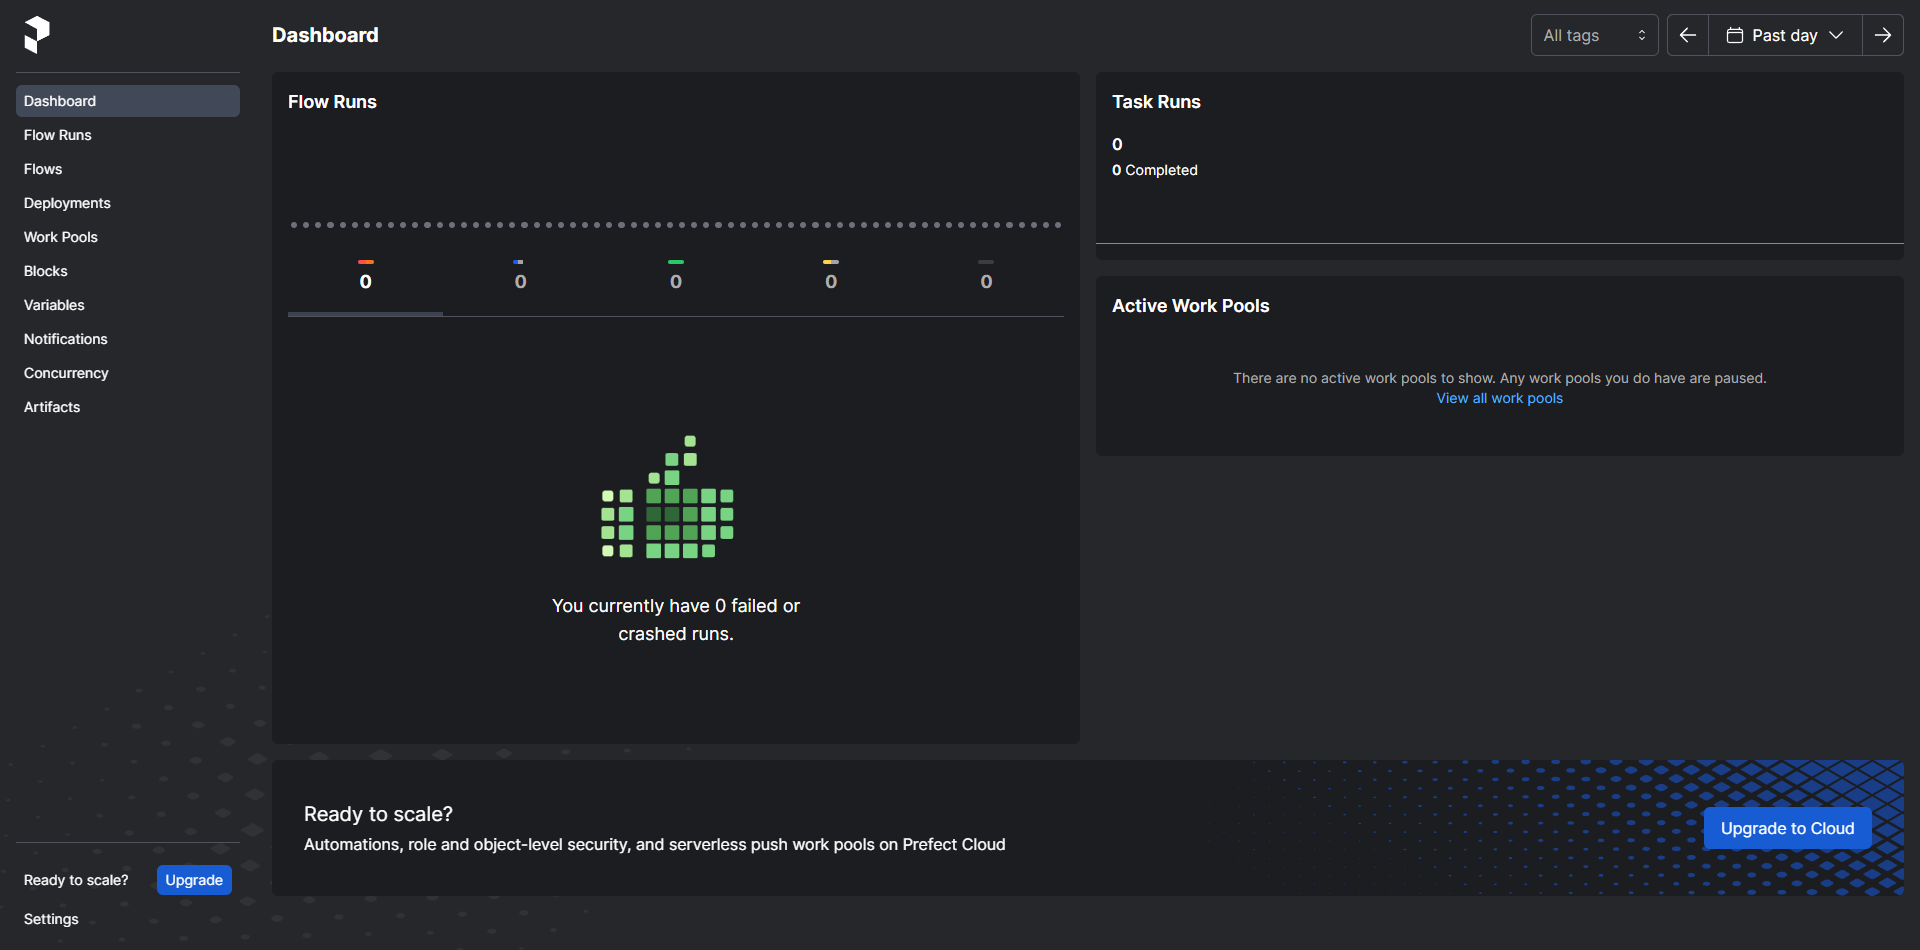
\includegraphics[width=\linewidth]{graphics/Prefect_dashboard.PNG}
    \caption{Prefect Dashboard}
    \label{fig:Prefect_Dashboard}
\end{figure}
De functies die gezien kunnen worden op figuur \ref{fig:Prefect_Dashboard} zijn:
\begin{itemize}
    \item Dashboard: Geeft een overzicht van alle flow runs, hier kan gekeken worden waneer een flow succesvol of onsuccesvol uitgevoerd werd.
    \item Flow Runs: Geeft een tijdlijn weer met alle flow die uitgevoerd zijn over een bepaalde tijd.
    \item Flows: Toont elke flow aan die in de code geschreven word. Hierbij kan ook in de flow gekeken worden om te zien welke taken het bevat.
    \item Deployments: Toont alle deployments weer, deze zijn flows die rechtstreeks met het dashboard kunnen worden uitgevoerd.
    \item Work Pools: Hier kan verbinding gemaakt worden met een externe infrastructuur zoals: Azure, AWS, Docker, echter
    \item Blocks: Hier word alle gevoelige informatie bijgehouden, zoals wachtwoorden en API keys.
    \item Work Pools: Hier kan er verbinding gemaakt worden met een cloud omgeving om de pipeline daar te laten uitvoeren.
\end{itemize}
Dit Proof of Concept zal gebruik maken van de ``Flow runs'' en ``Flows'' paginas op het dashboard.
\subsection{Uitvoering}
Prefect werkt met decorators, dit zorgt ervoor dat bestaande Python-functies makkelijk kunnen worden omgezet naar het Prefect framework. De twee decorators ``@task'' en ``@flow'' werd  eerder in de stand van zaken werd uitgelegd.
Deze maken het mogelijk om bestaande python functies om te zetten naar het Prefect framework.
\subsection{Preprocessing}
Orgineel was preprocessing het downloaden en het verwerken van de afbeeldingen maar voor het uitvoeren in Prefect is dit nog eens onderverdeeld geweest in twee aparte delen.
Het downloaden en het verwerken gebeurd dus apart. Als bijlage kan de Prefect code te zien zijn.
\subsection{Training}

\subsection{Evaluatie}

\subsection{Pipeline}
De pipeline in Prefect is een flow waarin alle tasks en flows achter elkaar worden uitgevoerd. De flow of pipeline ziet er als volgt uit:
\begin{minted}[frame=lines,breaklines,linenos]{python}
@flow(task_runner=SequentialTaskRunner(), log_prints=True)
def main():
    tracking_uri = "http://127.0.0.1:8080"
    model_name = "PoC"
    mlflow.set_tracking_uri(tracking_uri)
    mlflow.set_experiment(model_name)
    download()
    preprocess()
    model = train()
    eval(model)
\end{minted}

Deze code stelt eerst de juiste tracking adress in voor MLFlow en het model naam.
Hierna worden alle functies achter elkaar uitgevoerd en kunnen deze dan ook in de dashboard gezien worden zoals in figuur xxx.

In dit geval heeft de ``@flow'' nog extra parameters, deze betekenen:

% \begin{itemize}
%     \item task_runner: Geeft aan hoe dat de taken en flows moeten uitgevoerd worden, in dit geval is dat een ``SequentialTaskRunner'' wat betekend dat alle tasks en flows achter elkaar worden uitgevoerd.
%     \item log_prints: Geeft alle prints weer dat in de Python code werd gebruikt, in dit geval is dat ``True'' dat maakt het gemakkelijk tijden het ontwikkelen van de pipeline.
% \end{itemize}

Na het uitvoeren van de flow word deze flow gevisualiseerd in de web interface van Prefect. Figuur 
\subsection{Problemen}
Prefect had het moeilijk met het doorgeven van parameters naar de volgende ``Task''. Waardoor de flow niet meer kon werken, om dit op te lossen is er gebruik gemaakt van een subflow.
Subflows zijn flows die worden uitgevoerd in een bestaande flow. Deze ontvangen wel goed de parameters en kunnen alles goed uitvoeren.
\subsection{Cloud}
Prefect heeft een concept dat noemt ``Work Pools'' figuur \ref{fig:Prefect_Work_Pools} toont hoe dat deze pagina in Prefect eruit ziet:
\begin{figure}[h]
    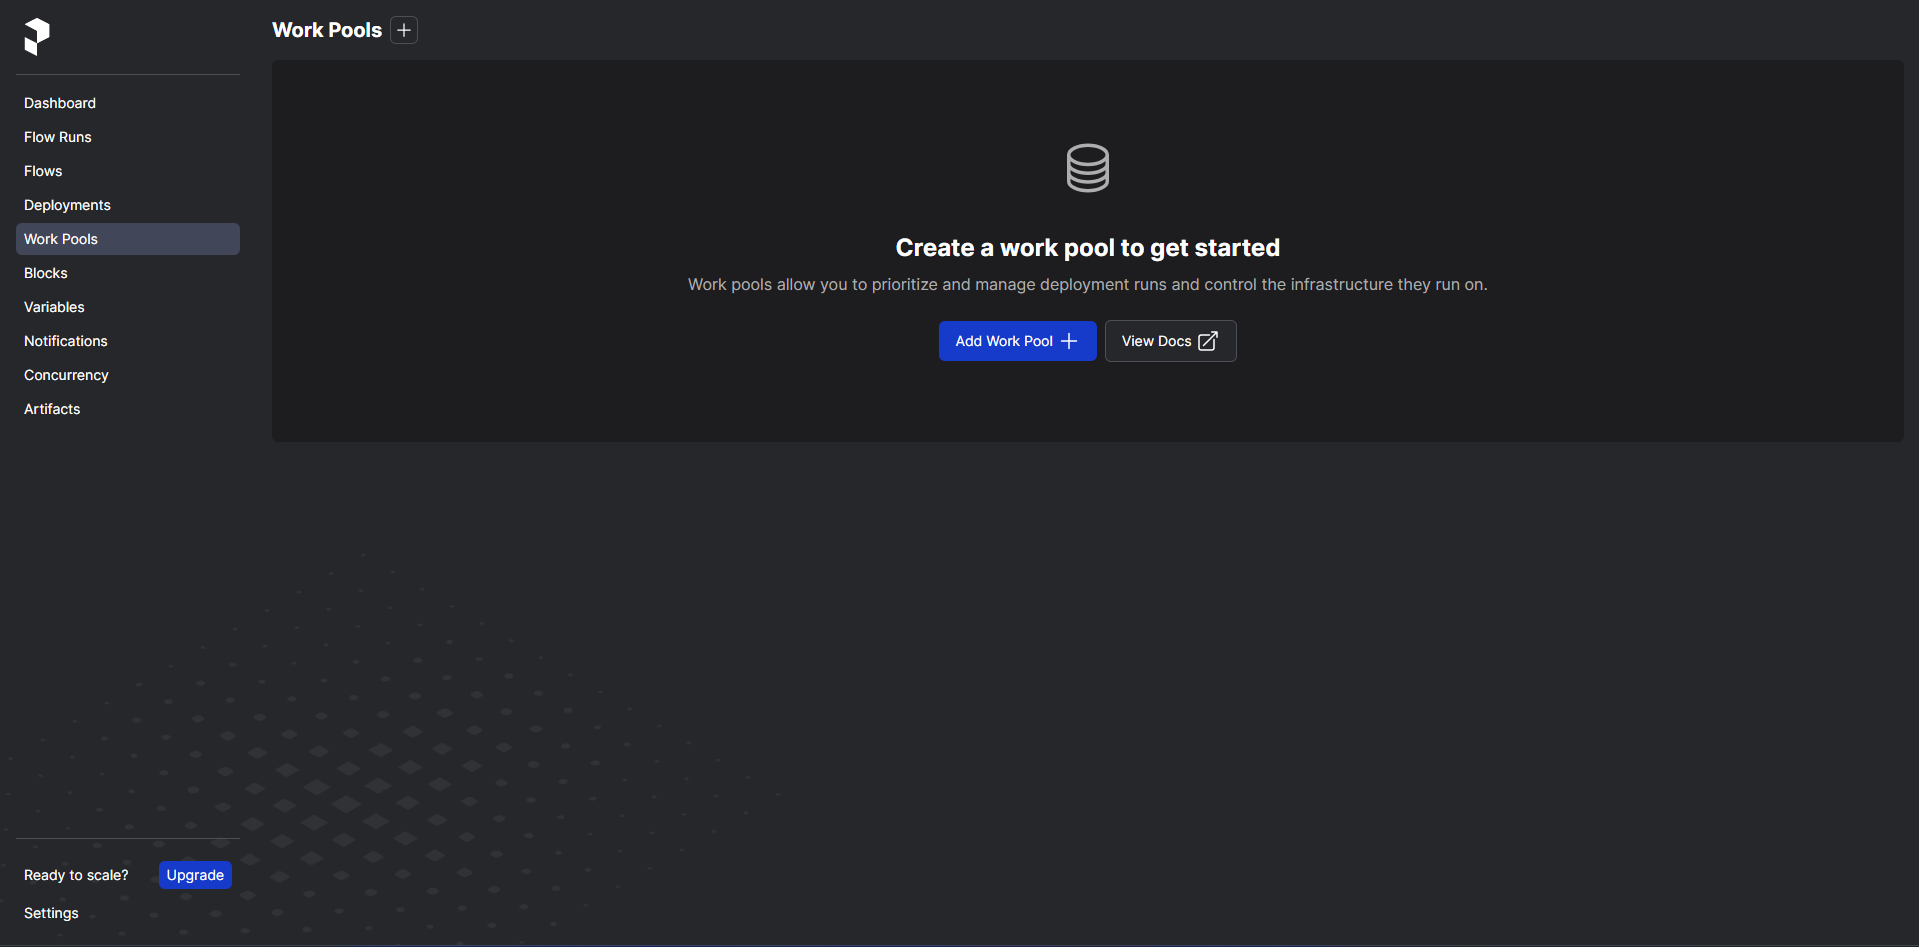
\includegraphics[width=\linewidth]{graphics/Prefect_Work_Pools.PNG}
    \caption{Prefect Work Pool Pagina}
    \label{fig:Prefect_Work_Pools}
\end{figure}
Op deze pagina kan er een ``Work Pools'' worden toegevoeg deze zorgen voor een connectie met een cloud omgeving, zodat de Prefect flow in de cloud kan worden uitgevoerd.
Het aanmaken van een verbinding kan via de knop ``Add Work Pool'' van figuur \ref{fig:Prefect_Work_Pools}.
Na het klikken van deze knop kan je kiezen met welke cloud omgeving dat er verbinding met gemaakt moet worden zoals te zien op figuur \ref{fig:Prefect_Work_Pools_Create}.
\begin{figure}[h]
    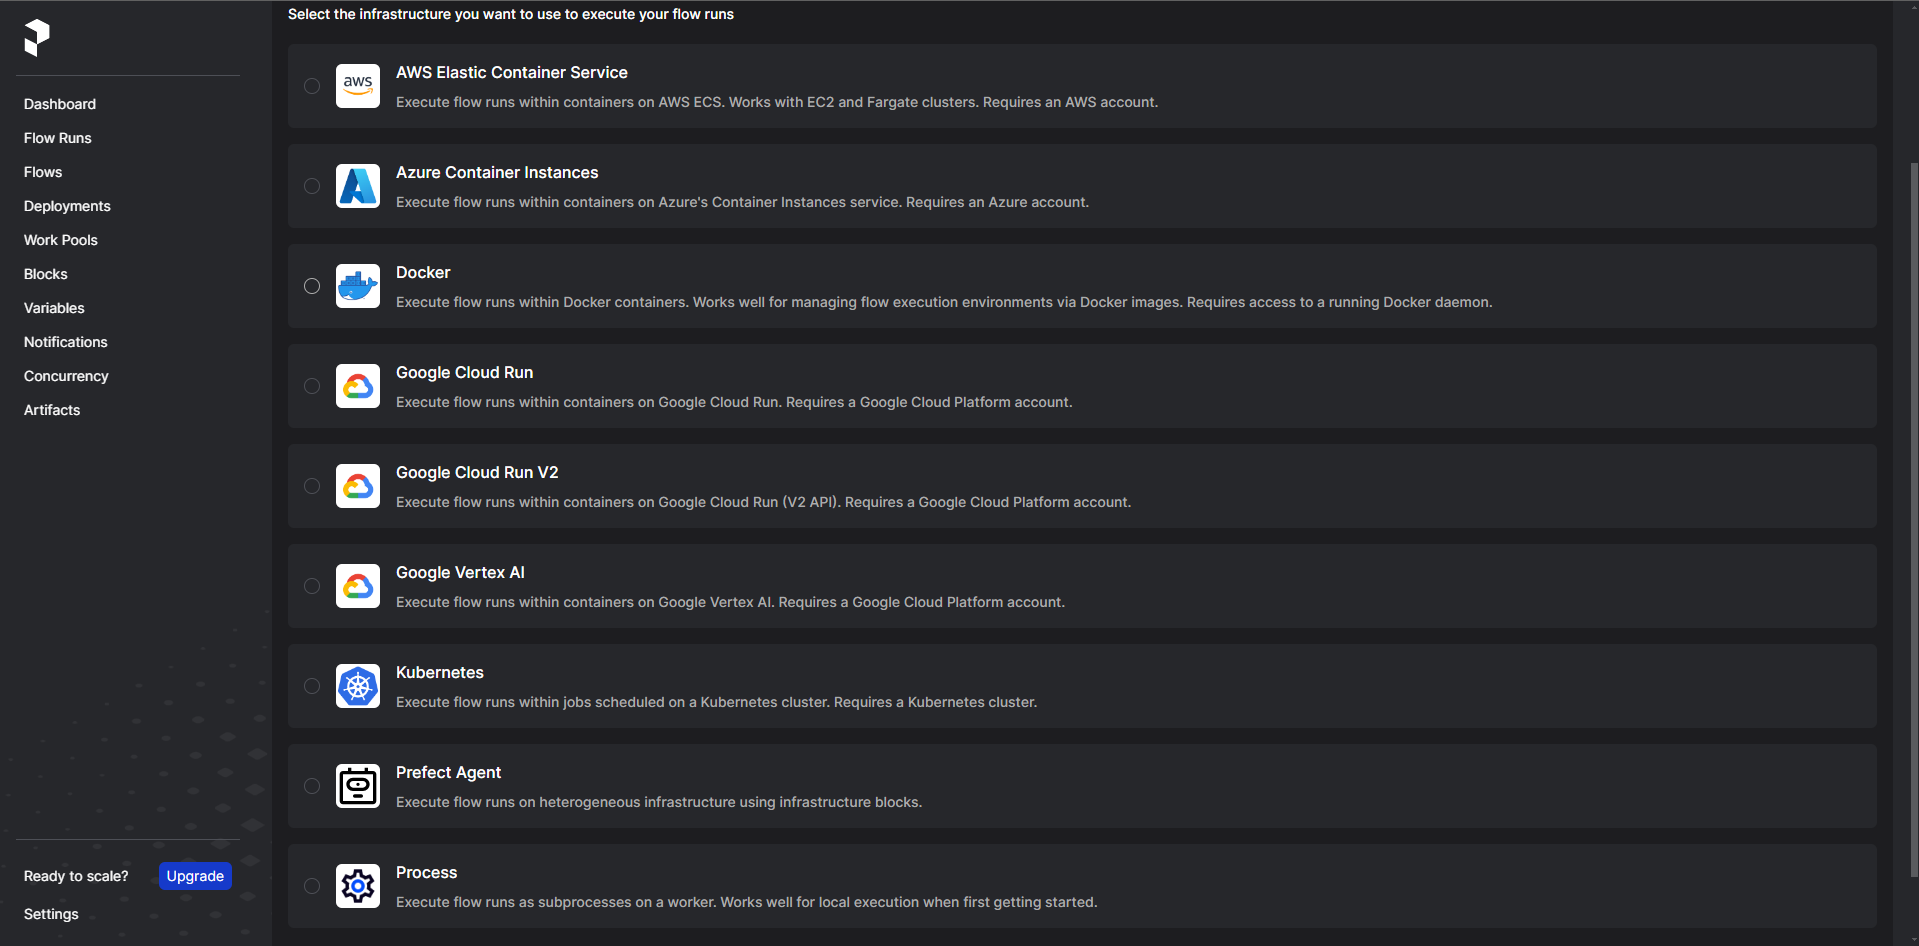
\includegraphics[width=\linewidth]{graphics/Prefect_Work_Pools_Create.PNG}
    \caption{Prefect Work Pool Cloud provider}
    \label{fig:Prefect_Work_Pools_Create}
\end{figure}
Figuur \ref{fig:Prefect_Work_Pools_Create} toont de verschillende cloud omgevingen waarmee dat Prefect kan werken. Deze zijn:
\begin{itemize}
    \item AWS Elastic Container Service
    \item Azure Container Instances
    \item Docker
    \item Google Cloud Run
    \item Google Cloud Run v2
    \item Google Vertex AI
    \item Kubernetes
    \item Prefect Agent 
    \item Process
\end{itemize}
Voor dit voorbeeld gaan we Process selecteren omdat er momenteel geen toegang is tot een cloud omgeving.
De volgende stap is het invullen van details, Deze details zijn de naam en de beschrijving van de ``Work Pool'' en eventuele Concurrency. Alleen de naam is verplicht om in te vullen zoals te zien in figuur \ref{fig:Prefect_Work_Pools_Create_Details}.
\begin{figure}[h]
    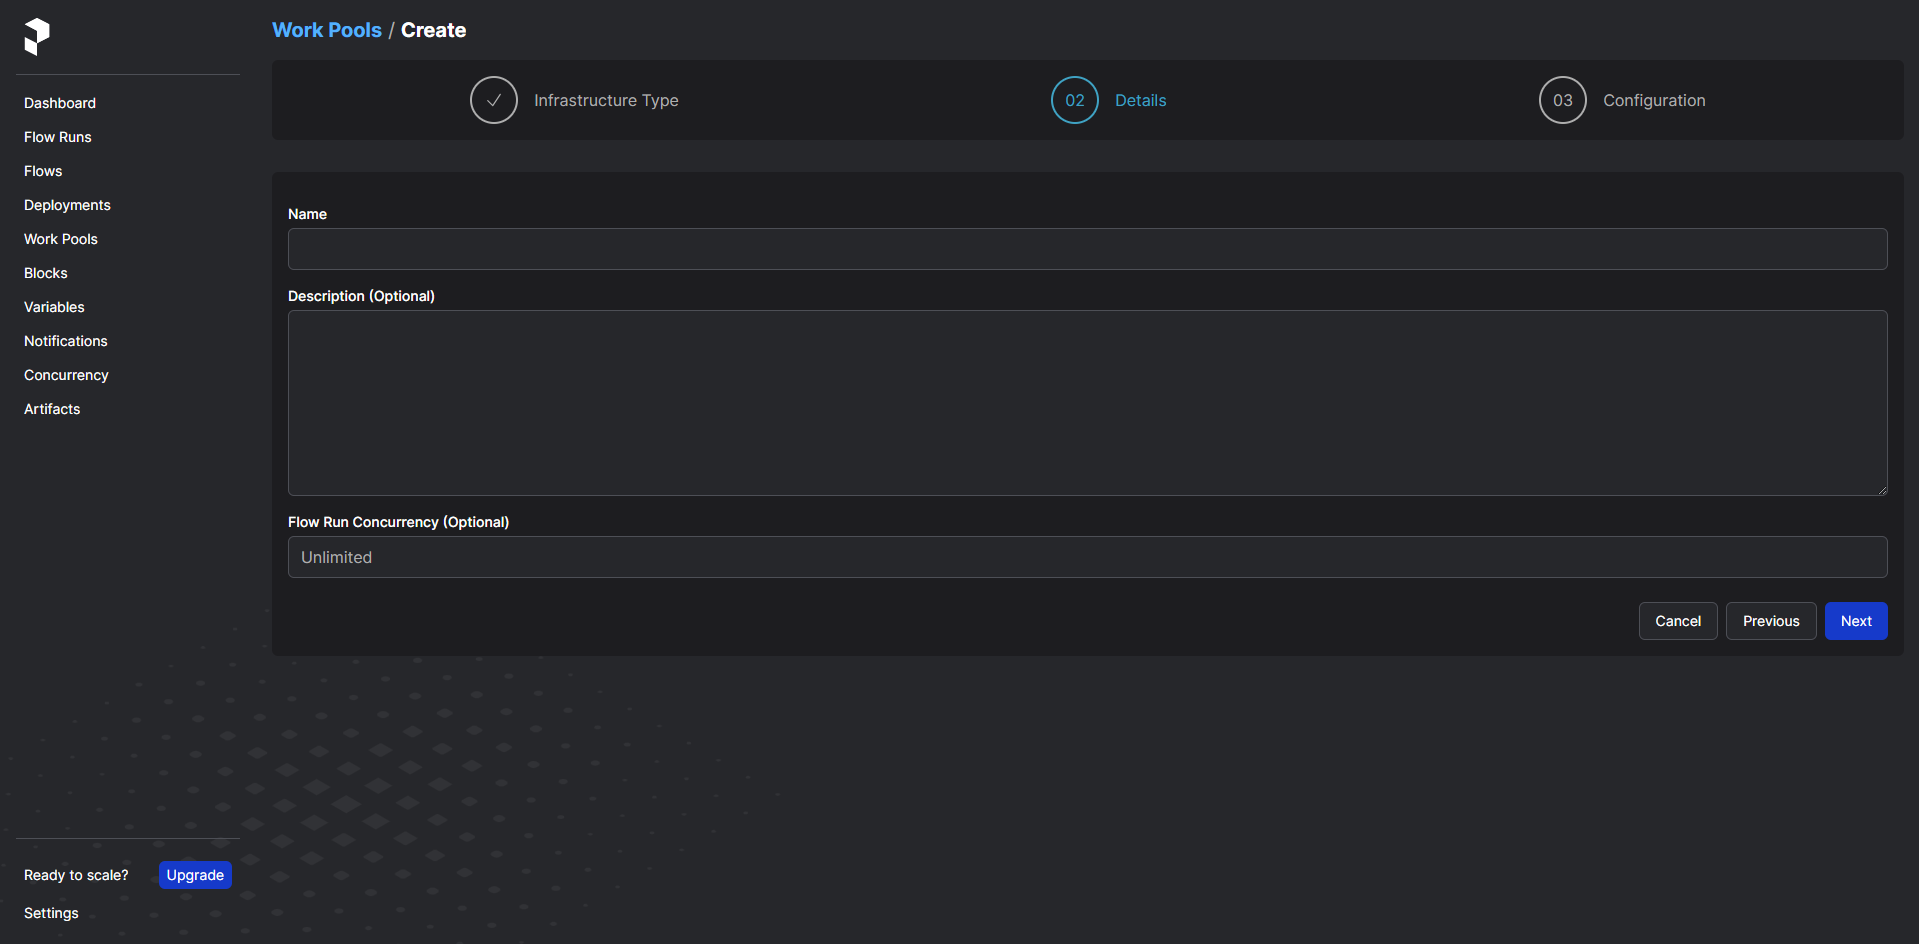
\includegraphics[width=\linewidth]{graphics/Prefect_Work_Pools_Create_Details.PNG}
    \caption{Prefect Work Pool Creation Details}
    \label{fig:Prefect_Work_Pools_Create_Details}
\end{figure}
Ten slotte op de laatste pagina worden extra parameters ingesteld in verband met de cloud provider, dit is te zien op figuur \ref{fig:Prefect_Work_Pools_Create_parameters}
\begin{figure}[h]
    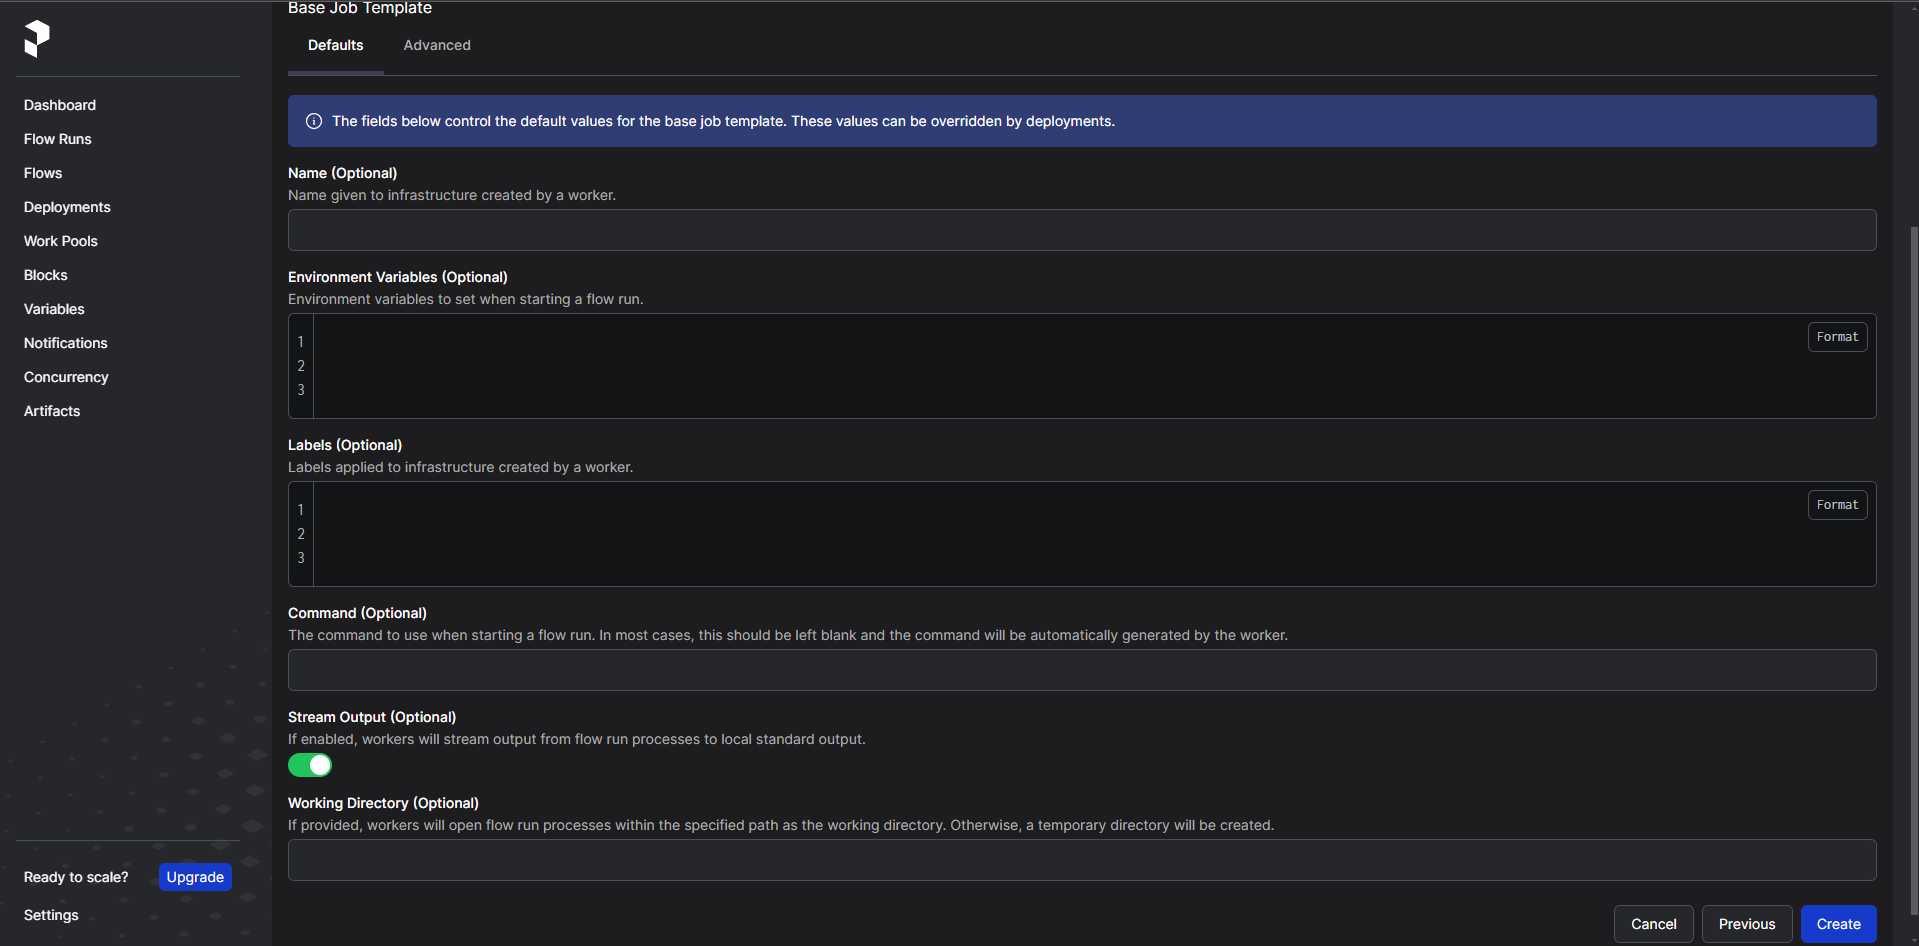
\includegraphics[width=\linewidth]{graphics/Prefect_Work_Pools_Create_Parameters.PNG}
    \caption{Prefect Work Pool Creation Details}
    \label{fig:Prefect_Work_Pools_Create_parameters}
\end{figure}
\section{ZenML}
\subsection{Installatie}
\subsection{Dashboard}
\subsection{Uitvoering}
\subsection{Pipeline}
\subsection{Problemen}
\subsection{Cloud}

\section{Dagster}
\subsection{Installatie}
\subsection{Dashboard}
\subsection{Uitvoering}
\subsection{Pipeline}
\subsection{Problemen}
\subsection{Cloud}


